\documentclass[10pt]{article}
\usepackage[margin=1in]{geometry}
\usepackage[T1]{fontenc}\usepackage{mathptmx}
\usepackage{amsmath,amssymb,booktabs,graphicx,caption,subcaption,hyperref,xcolor,microtype,enumitem}
\usepackage[numbers,sort&compress]{natbib}
\hypersetup{colorlinks,linkcolor=blue!50!black,citecolor=blue!50!black,urlcolor=blue!50!black}
\newcommand{\allFnc}{\$0.3865}
\newcommand{\allFc}{\$0.0819}
\newcommand{\cachedisc}{78.8\%}
\newcommand{\hNaive}{51.3\%}
\newcommand{\hNoCache}{50.8\%}
\newcommand{\hCache}{9.2\%}
\newcommand{\hRouted}{\$0.0744}
\newcommand{\hRoutedNc}{\$0.1901}
\newcommand{\sNaive}{33.8\%}
\newcommand{\sNoCache}{33.3\%}
\newcommand{\sCache}{$-$15.5\%}
\newcommand{\sRouted}{\$0.0947}
\newcommand{\sRoutedNc}{\$0.2580}
\newcommand{\bigShare}{30.9\%}
\newcommand{\missTurn}{0.8\%}
\newcommand{\hSticky}{$-$0.2\%}
\newcommand{\sSticky}{$-$10.4\%}
\newcommand{\stickyShare}{77.9\%}
\newcommand{\mcFive}{$-$3.4\%}
\newcommand{\mcMed}{6.5\%}
\newcommand{\mcNinetyFive}{18.3\%}
\newcommand{\mcNaive}{46.7\%}
\newcommand{\mcGap}{40.2}
\newcommand{\mcNeg}{16.2\%}
\newcommand{\mcMiss}{1.0\%}
\newcommand{\mcMissHi}{3.5\%}
\newcommand{\mcN}{600}
\newcommand{\allHaiku}{70.0\%}
\newcommand{\allSonnet}{39.9\%}
\newcommand{\allHaikuCost}{\$0.0246}
\newcommand{\allSonnetCost}{\$0.0492}
\newcommand{\noHard}{18.4\%}
\newcommand{\convCeiling}{12.9\%}
\newcommand{\valGap}{1.1}
\newcommand{\heatLo}{$-$0.3\%}
\newcommand{\heatHi}{21.0\%}
\newcommand{\rhoPI}{$-0.52$}
\newcommand{\rhoTPR}{$-0.02$}
\newcommand{\rhoFPR}{$-0.52$}
\newcommand{\rhoS}{$-0.22$}
\newcommand{\rhoT}{$+0.24$}
\newcommand{\rhoO}{$+0.47$}
\newcommand{\spA}{$-$11.1\%}
\newcommand{\spB}{3.8\%}
\newcommand{\spC}{11.0\%}
\newcommand{\spD}{7.5\%}

\newcommand{\pin}{p^{\mathrm{in}}}\newcommand{\pout}{p^{\mathrm{out}}}

\title{\textbf{When Caching Meets Routing:}\\A Cache-Aware Cost Model for Selective Frontier-Model Routing in Multi-Turn Voice Agents}
\author{Michael Kaminski\\\small Modular Equity, Atlanta, GA\\\small\texttt{michael@modularequity.com}}
\date{Technical white paper \quad\textperiodcentered\quad September 28, 2026 \quad\textperiodcentered\quad Preprint, not peer-reviewed}

\begin{document}
\maketitle

\begin{abstract}
\noindent Routing the easy turns in an LLM workload to a cheaper model and saving the frontier model for hard turns is widely reported to cut inference cost by 35--98\% at near-frontier quality \cite{chen2023frugalgpt,ong2024routellm,ding2024hybrid}. These estimates generally treat each query as independent and priced at list rates. Multi-turn conversational agents, such as contact-center voice agents, break both assumptions: every turn re-sends a long, mostly unchanged context, and providers bill the re-sent prefix at a steep discount through \emph{prompt caching}. Caches, however, are kept per model. We build a turn-level simulator that combines published prices (retrieved 2026-09-28), prompt-cache rules, a Markov process for turn difficulty, and an imperfect router with escalation. With caching switched off, it reproduces a closed-form list-price model to within \valGap{} percentage points. Under a representative baseline (12 turns, 6{,}000-token cached system prompt, 20\% hard turns), per-turn routing from Claude Opus~5.5 to Haiku~4.5 saves \hNaive{} under the naive model but only \hCache{} once caching is modeled. Routing Opus~5.5 to Sonnet~5.5 moves from \sNaive{} savings to a net cost \emph{increase} of \sCache{}. Across \mcN{} Monte Carlo scenarios, median cache-aware savings are \mcMed{} (90\% interval \mcFive{} to \mcNinetyFive{}), against a naive median of \mcNaive{}. Routing loses money in \mcNeg{} of scenarios. The cause is \emph{cache fragmentation}: tokens appended while a model is idle must be re-written to that model's cache at $1.25\times$ input price. Routing whole conversations instead of individual turns avoids the penalty and recovers up to \allHaiku{} savings on conversations routed to the small model. Every number in this paper is regenerated by a public script, and no proprietary or employer data is used.
\end{abstract}

\section{Introduction}
\paragraph{What we mean by ``frontier.''} A \emph{frontier model} is a general-purpose model at the current edge of capability. It is usually trained with the largest compute budgets and leads broad reasoning, coding and agentic benchmarks. Architecture (transformer, matrix-multiply-heavy) does not define the class, because nearly every modern neural network shares it. Frontier models are also typically the \emph{slowest and most expensive per token}, not the fastest. Regulators have drawn the boundary by training compute; the EU AI Act, for example, presumes systemic risk above $10^{25}$ FLOPs \cite{euaiact}. This definition matters because the obvious cost strategy for production agents follows from it: use the frontier model only where its capability is needed.

\paragraph{The routing thesis.} LLM routing and cascading try to do exactly that. FrugalGPT reports up to 98\% cost reduction while matching GPT-4 \cite{chen2023frugalgpt}. RouteLLM reports cost reductions of over 85\% on MT-Bench, 45\% on MMLU and 35\% on GSM8K while keeping 95\% of GPT-4's quality \cite{ong2024routellm,lmsys2024routellm}. Hybrid LLM reports up to 40\% fewer calls to the large model with no drop in quality \cite{ding2024hybrid}. RouterBench supplies over 405k inference outcomes for evaluating routers \cite{hu2024routerbench}. These results are real, but they come from \emph{single-turn} benchmarks priced at \emph{list} rates.

\paragraph{The gap.} A voice agent in collections or servicing is multi-turn by construction. Each turn re-sends a system prompt, tool schemas, policy text and the growing transcript. Providers discount a re-sent prefix heavily: Anthropic bills cache reads at $0.05$--$0.1\times$ base input price \cite{anthropiccache}. A cache hit requires an identical prefix, and the cached state is the attention keys and values computed by one model, so a cache written by one model cannot be read by another: caches are, in effect, \emph{isolated per model}. We therefore ask:
\begin{quote}\itshape
How much of the routing savings reported in the literature survives in a multi-turn agent once prompt caching and per-model cache isolation are modeled?
\end{quote}

\paragraph{Contributions.}
\begin{enumerate}[leftmargin=*,itemsep=1pt]
\item A turn-level, cache-aware cost model for routed multi-turn agents (\S\ref{sec:model}), checked against a closed-form list-price model with caching switched off.
\item Evidence that caching removes most per-turn routing savings, and that routing can \emph{raise} cost when the cheaper model's cache-read price is not lower (\S\ref{sec:results}).
\item A named mechanism, \emph{cache fragmentation}, and a design rule: route at the granularity of the cache (the conversation), not the turn (\S\ref{sec:discussion}).
\end{enumerate}

\section{Background: pricing and caching}\label{sec:bg}
Table~\ref{tab:prices} lists the public prices used. Two facts drive the results. First, the list-price ratio between the frontier and small model is $4\times$ (Opus~5.5 to Haiku~4.5) or $2\times$ (Opus~5.5 to Sonnet~5.5), but the cache-read ratio is only $2\times$ and $1\times$, because Opus~5.5 reads its cache at a reduced $0.05\times$ multiplier. Second, a cache hit requires an identical prefix, in practice on the \emph{same model}, lasts 5 minutes by default (refreshed on use), and costs $1.25\times$ input to write. Haiku~4.5 will not cache prompts shorter than 4{,}096 tokens \cite{anthropiccache}.

\begin{table}[h]\centering\small
\caption{Anthropic list prices, USD per million tokens, retrieved 2026-09-28 \cite{anthropicpricing,anthropiccache}.}\label{tab:prices}
\begin{tabular}{lrrrrr}\toprule
Model & Input & Output & Cache write (5\,min) & Cache read & Min.\ cacheable tokens\\\midrule
Claude Opus 5.5 (frontier) & 4.00 & 20.00 & 5.00 & 0.20 & 512\\
Claude Sonnet 5.5 & 2.00 & 10.00 & 2.50 & 0.20 & 512\\
Claude Haiku 4.5 & 1.00 & 5.00 & 1.25 & 0.10 & 4{,}096\\\bottomrule
\end{tabular}\end{table}

\section{Model}\label{sec:model}
\paragraph{Conversation.} A conversation has $T$ turns. The prompt at turn $t$ has length $L_t = S + \sum_{k<t}(u+o+\tau_k) + u$, where $S$ is the static system-plus-tools prefix, $u$ the caller utterance, $o$ the agent response and $\tau_k$ the tool-result tokens.

\paragraph{Turn difficulty.} Hard turns (those that need frontier reasoning) follow a two-state Markov chain with persistence $\phi=\Pr(h_t=1\mid h_{t-1}=1)$ and stationary share $\pi$. This requires $\Pr(h_t=1\mid h_{t-1}=0)=\pi(1-\phi)/(1-\pi)$.

\paragraph{Router.} On every turn a small classifier call (200 input and 5 output tokens on Haiku~4.5) flags the turn as hard with probability $\mathrm{TPR}$ if it is hard and $\mathrm{FPR}$ if it is easy. Flagged turns go to the frontier model $F$ and unflagged turns go to the small model $s$. A hard turn sent to $s$ is caught by a self-check with probability $e$ and re-answered by $F$, so both calls are billed. Otherwise it is \emph{missed}, which is a quality loss.

\paragraph{Naive (list-price) model.} If caching and router cost are ignored and $\rho = \pout_s/\pout_F$ (equal to $\pin_s/\pin_F$ for these pairs), expected cost relative to frontier-only is
\begin{equation}\label{eq:naive}
\kappa = \pi\big[\mathrm{TPR} + (1-\mathrm{TPR})(\rho+e)\big] + (1-\pi)\big[\mathrm{FPR} + (1-\mathrm{FPR})\rho\big],\qquad \text{savings} = 1-\kappa .
\end{equation}

\paragraph{Cache-aware model.} Let $\ell_m$ be the warm prefix for model $m$: the prompt length at $m$'s previous call if that call was within the TTL, and $0$ otherwise. One call to $m$ costs
\begin{equation}\label{eq:call}
c_m(L,\ell_m) = \begin{cases}\ell_m\, r_m + (L-\ell_m)\, w_m + o\,\pout_m, & L \ge L^{\min}_m\\[2pt] L\,\pin_m + o\,\pout_m, & \text{otherwise,}\end{cases}
\end{equation}
where $r_m$ and $w_m=1.25\,\pin_m$ are the cache read and write prices. We assume the whole prompt is cached on every call, which is standard for multi-turn agents.

\paragraph{Cache fragmentation.} Under frontier-only operation, each turn writes only the $\approx u+o+\tau$ new tokens. Under routing, when $F$ returns after $k$ turns on $s$, it must write every token appended during those $k$ turns, $\Delta_F=\sum_{j}(u+o+\tau_j)$, at $w_F$ instead of $r_F$. The small model likewise pays to write the full prefix $S$ once. We call the extra write cost the \emph{fragmentation penalty}. Eq.~\eqref{eq:naive} leaves it out.

\section{Experimental setup}
Table~\ref{tab:params} lists the baseline and Monte Carlo ranges. The parameters are \emph{assumptions} chosen to represent a contact-center voice agent. They are not measurements from any deployment. Each point estimate averages 4{,}000 simulated conversations (fixed seeds). The Monte Carlo study draws \mcN{} parameter vectors uniformly from the ranges and simulates 60 conversations for each.

\begin{table}[h]\centering\small
\caption{Simulation parameters (assumptions).}\label{tab:params}
\begin{tabular}{llcc}\toprule
Symbol & Meaning & Baseline & MC range\\\midrule
$T$ & turns per conversation & 12 & 6--20\\
$S$ & static cached prefix (system, tools, policy) & 6{,}000 & 4{,}500--12{,}000\\
$u,\ o$ & caller / agent tokens per turn & 60, 80 & 30--100, 40--150\\
$\bar\tau$ & mean tool-result tokens per turn (on 50\% of turns) & 150 & 0--400\\
$\pi,\ \phi$ & hard-turn share, persistence & 0.20, 0.5 & 0.10--0.40, 0.2--0.8\\
TPR, FPR & router true/false positive rate & 0.90, 0.15 & 0.80--0.97, 0.05--0.30\\
$e$ & self-check escalation rate for missed hard turns & 0.6 & 0.3--0.8\\
--- & seconds per turn; cache TTL & 20; 300 & fixed\\\bottomrule
\end{tabular}\end{table}

\section{Results}\label{sec:results}
\paragraph{Validation.} With caching switched off, the simulator reproduces Eq.~\eqref{eq:naive} to within \valGap{} percentage points for every $\pi\in[0.05,0.6]$ and both model pairs (Fig.~\ref{fig:pi}, grey vs.\ dashed). For example, it gives \hNoCache{} simulated against \hNaive{} analytic at baseline. The remaining gap is the router's own cost. This checks the routing and escalation arithmetic, not the cache-billing path, which rests on the published pricing rules in \S\ref{sec:bg}.

\paragraph{Caching alone.} Prompt caching cuts frontier-only cost from \allFnc{} to \allFc{} per conversation, a \cachedisc{} reduction. This single, near-free change dwarfs what any router can add at baseline.

\begin{table}[h]\centering\small
\caption{Baseline cost per conversation and savings versus frontier-only. The negative value marks a cost increase.}\label{tab:base}
\begin{tabular}{lcccc}\toprule
& \multicolumn{2}{c}{No caching} & \multicolumn{2}{c}{Cache-aware}\\\cmidrule(lr){2-3}\cmidrule(lr){4-5}
Policy & Cost & Savings & Cost & Savings\\\midrule
Frontier-only (Opus 5.5) & \allFnc & --- & \allFc & ---\\
Per-turn route $\to$ Haiku 4.5 & \hRoutedNc & \hNoCache & \hRouted & \hCache\\
Per-turn route $\to$ Sonnet 5.5 & \sRoutedNc & \sNoCache & \sRouted & \sCache\\
Sticky escalation $\to$ Haiku 4.5 & --- & --- & --- & \hSticky\\
Whole conversation on Haiku 4.5 & --- & --- & \allHaikuCost & \allHaiku\\
Whole conversation on Sonnet 5.5 & --- & --- & \allSonnetCost & \allSonnet\\\bottomrule
\end{tabular}\end{table}

\paragraph{Routing under caching.} Table~\ref{tab:base} and Fig.~\ref{fig:pi} show the main result. Per-turn routing to Haiku~4.5 sends \bigShare{} of turns to the frontier model and misses \missTurn{} of turns. Its savings fall from \hNoCache{} to \hCache{} once caching is modeled. Routing to Sonnet~5.5 \emph{raises} cost by \textbf{\sCache{}}, because Sonnet~5.5 reads its cache at the same \$0.20/MTok as Opus~5.5, so fragmentation writes outweigh the output-price savings. Fig.~\ref{fig:decomp} breaks the cost down: routing halves output spend, but cache-write spend \emph{grows}.

\begin{figure}[h]\centering
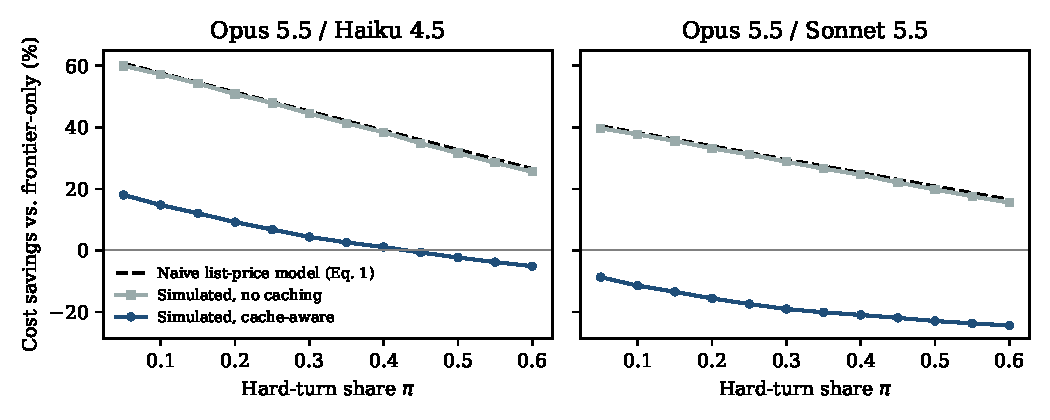
\includegraphics[width=\linewidth]{figures/savings_vs_pi.pdf}
\caption{Savings versus hard-turn share $\pi$. Dashed: Eq.~\eqref{eq:naive}. Grey: simulator with caching off (validation). Blue: cache-aware simulator.}\label{fig:pi}
\end{figure}

\begin{figure}[h]\centering
\begin{subfigure}{.48\linewidth}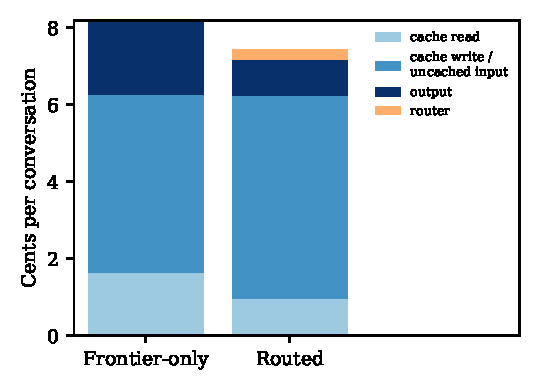
\includegraphics[width=\linewidth]{figures/decomp.pdf}\caption{Cost decomposition, Opus 5.5/Haiku 4.5.}\label{fig:decomp}\end{subfigure}\hfill
\begin{subfigure}{.48\linewidth}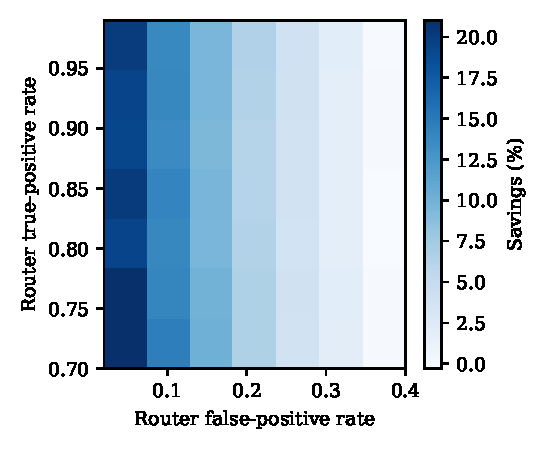
\includegraphics[width=\linewidth]{figures/heat.pdf}\caption{Savings by router TPR and FPR ($\pi=0.2$).}\label{fig:heat}\end{subfigure}
\caption{Where routing savings come from, and how much router quality matters.}\end{figure}

\paragraph{Router quality.} Across $\mathrm{TPR}\in[0.70,0.99]$ and $\mathrm{FPR}\in[0.02,0.40]$, cache-aware savings range from \heatLo{} to \heatHi{} (Fig.~\ref{fig:heat}). The false-positive rate matters far more than the true-positive rate. Every false positive pays full frontier price \emph{and} a fragmentation write.

\paragraph{Uncertainty.} Across \mcN{} scenarios, cache-aware savings have a median of \mcMed{} and a 90\% interval of \mcFive{} to \mcNinetyFive{}. The naive model's median is \mcNaive{}, so it overstates savings by a median of \mcGap{} percentage points (Fig.~\ref{fig:mc}). Routing increases cost in \mcNeg{} of scenarios. The median missed-hard-turn rate is \mcMiss{} (95th percentile \mcMissHi{}). Spearman correlations with savings are: FPR \rhoFPR, $\pi$ \rhoPI, agent output length $o$ \rhoO, turns $T$ \rhoT, prefix $S$ \rhoS, TPR \rhoTPR. Routing pays best when output makes up a large share of cost and the cached prefix is small.

\begin{figure}[h]\centering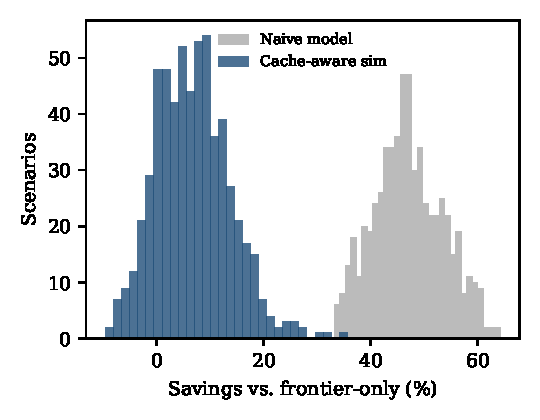
\includegraphics[width=.5\linewidth]{figures/mc.pdf}
\caption{Distribution of savings across \mcN{} parameter draws: naive model (grey) and cache-aware simulator (blue).}\label{fig:mc}\end{figure}

\paragraph{Alternative policies.} \emph{Sticky escalation} keeps a conversation on the frontier model once it has escalated, and stops calling the router. It avoids fragmentation but drifts \stickyShare{} of turns to $F$, giving \hSticky{} (Haiku) and \sSticky{} (Sonnet). \emph{Conversation-level routing} keeps each cache intact. A conversation served entirely by Haiku~4.5 costs \allHaiku{} less than one on Opus~5.5. Realized savings then equal \allHaiku{} times the share of conversations that can safely be assigned to the small model up front. At baseline, \noHard{} of conversations contain no hard turn, which caps savings at about \convCeiling{} even with a perfect conversation-level classifier.

\paragraph{Short prefixes.} When $S$ is below Haiku~4.5's 4{,}096-token caching minimum, early small-model calls cannot be cached. Per-turn routing savings are \spA{} at $S{=}2{,}000$, \spB{} at 3{,}500, \spC{} at 4{,}500 and \spD{} at 8{,}000.

\section{Discussion: design implications}\label{sec:discussion}
\begin{enumerate}[leftmargin=*,itemsep=2pt]
\item \textbf{Cache first, route second.} Caching delivered a \cachedisc{} reduction in this setting. Any routing business case should be measured against a \emph{cached} frontier-only baseline, not list prices.
\item \textbf{Compare effective prices, not list prices.} The relevant ratio blends cache-read, cache-write and output prices, weighted by the workload's token mix. A cheaper model with the same cache-read price (here Sonnet~5.5) can be a net loss.
\item \textbf{Route at cache granularity.} Assigning whole conversations, or long stable segments, avoids fragmentation. Per-turn routing should be limited to cases where the frontier call can be made \emph{stateless}, with a short, cacheable, model-specific prompt.
\item \textbf{Optimize FPR.} A router tuned for recall pays twice for every false alarm.
\item \textbf{Keep deterministic work off LLMs.} Calculations, policy lookups and state updates cost nothing to route and belong in code.
\end{enumerate}

\section{Limitations and threats to validity}
\begin{itemize}[leftmargin=*,itemsep=1pt]
\item \textbf{Assumed workload.} All token counts, difficulty rates and router accuracies are assumptions, not measurements. We encourage readers to replace them with their own traces.
\item \textbf{One provider's prices.} Other providers use different cache multipliers, TTLs and isolation rules, and prices change often. The mechanism generalizes, but the magnitudes may not.
\item \textbf{Quality as a proxy.} Quality is measured only as a missed-hard-turn rate; we do not score response quality.
\item \textbf{Speech costs excluded.} Speech-to-text, text-to-speech and telephony costs are omitted. They lower the share of LLM spend in total cost per call.
\item \textbf{No invoice check.} The cache-aware cost path is derived from published billing rules and has not been reconciled against real API invoices.
\item \textbf{Simplified caching.} We assume the whole prompt is cached on every call, with one breakpoint and a 5-minute TTL. More aggressive cache engineering could reduce the fragmentation penalty.
\end{itemize}

\section{Conclusion}
Published routing savings are measured on single-turn, list-priced benchmarks. Carried over to multi-turn agents, they overstate savings by a median of \mcGap{} percentage points in our scenarios, and can reverse sign. The cause is cache fragmentation across isolated per-model caches. The practical rule is to cache first, compare effective prices, and route at the granularity of the cache.

\paragraph{Reproducibility.} \texttt{model.py} regenerates every figure and \texttt{results.json}; \texttt{macros.py} writes every number in the text into \texttt{numbers.tex}. The model uses Python~3 with NumPy, SciPy and Matplotlib.

\paragraph{Disclosure.} The author leads a voice-AI initiative in consumer-finance servicing. This paper uses \emph{no} employer data, systems or results. All inputs are public prices or stated assumptions.

\begin{thebibliography}{9}
\bibitem[Chen et~al.(2023)]{chen2023frugalgpt} L.~Chen, M.~Zaharia, J.~Zou. FrugalGPT: How to use large language models while reducing cost and improving performance. arXiv:2305.05176, 2023.
\bibitem[Ong et~al.(2024)]{ong2024routellm} I.~Ong, A.~Almahairi, V.~Wu, W.-L.~Chiang, T.~Wu, J.~E.~Gonzalez, M.~W.~Kadous, I.~Stoica. RouteLLM: Learning to route LLMs with preference data. arXiv:2406.18665, 2024.
\bibitem[LMSYS(2024)]{lmsys2024routellm} LMSYS Org. RouteLLM: An open-source framework for cost-effective LLM routing. \url{https://www.lmsys.org/blog/2024-07-01-routellm/}, July 2024.
\bibitem[Ding et~al.(2024)]{ding2024hybrid} D.~Ding, A.~Mallick, C.~Wang, R.~Sim, S.~Mukherjee, V.~R\"uhle, L.~V.~S.~Lakshmanan, A.~H.~Awadallah. Hybrid LLM: Cost-efficient and quality-aware query routing. ICLR 2024. arXiv:2404.14618.
\bibitem[Hu et~al.(2024)]{hu2024routerbench} Q.~J.~Hu, J.~Bieker, X.~Li, N.~Jiang, B.~Keigwin, G.~Ranganath, K.~Keutzer, S.~K.~Upadhyay. RouterBench: A benchmark for multi-LLM routing system. arXiv:2403.12031, 2024.
\bibitem[Anthropic(2026a)]{anthropicpricing} Anthropic. Pricing. \url{https://platform.claude.com/docs/en/about-claude/pricing}, accessed 2026-09-28.
\bibitem[Anthropic(2026b)]{anthropiccache} Anthropic. Prompt caching. \url{https://platform.claude.com/docs/en/build-with-claude/prompt-caching}, accessed 2026-09-28.
\bibitem[EU(2024)]{euaiact} Regulation (EU) 2024/1689 (Artificial Intelligence Act), Art.~51. Official Journal of the European Union, 2024.
\end{thebibliography}
\end{document}
